\clearpage
\section{Method}
\label{sec:Method}

In a heterogeneous fleet of vehicles that is typically deployed by a car-sharing operator,
having insights of the features determining the vehicle choice of a customer is key
to operate in an efficient manner. This includes features like availability, travel-time
and driving distance, but also socio-demographic features of the area in which the
car-sharing system is deployed. During this study we will develop a classifier which 
captures this relation and use it to analyze an inter-area connected network of stations
during a discrete event driven simulation phase to get insights on performance critical
metrics.

\subsection{Concepts}
\label{sub_sec:Method/Concepts}

Firstly a set of concepts is defined, that will be important in the further discussion.

\subsubsection{Vehicle Classes}
\label{sub_sec:Method/Concepts/Classes}

Since we are analyzing a fleet of heterogeneous vehicles, we define the set of vehicle
classes $\mathbb{C}$, to be the set of possible vehicle choices a customer can make. A
discrete example of these vehicle classes can be found in the case study later on. These
classes are also used to determine the pricing of a trip. An implementation of this
framework is expected to define a pricing function:
$$
\text{cost}: \mathbb{C} \times  \mathbb{R} \to \mathbb{R}
$$
where the input is the rented class and the time traveled in minutes and the output is the
cost in local currency.

\subsubsection{Area}
\label{sub_sec:Method/Concepts/Area}

An area is an approximation of different socio-demographic distributions with regard to 
distinct categories, such as age, income or marital status. Formally a category is defined by the random variable $X$ which
comes from an unknown distribution with value range $K$. For the framework $X$ is then
captured in terms of probability of lying in specific
subclasses $R_K$, where $R_K$ is a partition of $K$, meaning that
$\bigcup_{r \in R} r = K$ and $a \cap b = \emptyset \ \forall a, b \in R$. Leading to the
specification of the distribution of $X$ for our framework:
$$
Z_X = \{ (r, P(X \in r)) \ |\ r \in R \}
$$
These values are sourced by empirical studies and are specified in the actual implementation
of the proposed framework.
Due to the fact that $R$ is a partition of $K$ the following invariant must hold true: $\sum_{z \in Z_X} z = 1$.
An area is then defined in terms of the set of categories $\mathbb{X}$ that are analyzed in the implementation 
and can therefore be described as:
$$
a = \{ Z_X \ | \ \forall X \in \mathbb{X} \}
$$

\subsubsection{Station}
\label{sub_sec:Method/Concepts/Station}

The Station is an important concept for the simulation stage of the proposed framework. A station is always
inside a particular area, namely there exists a function $\text{area}(s)$ which returns the area that the 
station is placed in. Additionally, a station has a state that is kept and updated throughout the simulation
stage, this includes a function which for every time $t \in \mathbb{R}$ and class $c \in \mathbb{C}$ returns
the delta of cars of class $c$ rented up until that time: $\Delta_s: \mathbb{R} \times \mathbb{C} \to \mathbb{N}$. This function
is bounded by the parameter $C$ (Capacity), such that $\Delta_s(t, c) \ge -C \ \forall t \in \mathbb{R} \land c \in \mathbb{C}$.
Representing the inability to satisfy customer requests after a maximum capacity is reached.

Leading to the spatial structure of the simulation environment, that is a fully connected graph where the nodes are 
the set of all stations in the simulation, called $\mathbb{S}$, and the edges of that graph called $\mathbb{E}$. An implementation
is required to provide a distance mapping $L: \mathbb{E} \to \mathbb{R}$, providing weights for the edges of the graph.

\subsubsection{Customer Request}
\label{sub_sec:Method/Concepts/Request}

Another crucial part is the customer request $r$, since that is the data that we will train on and use in the simulation
environment to structure new requests. Prior to deciding on the vehicle class a user has knowledge about
the starting station $s_{r, 0}$ and end station $s_{r, 1}$ that he/she wants to travel between. The request is also expected
to be sourced at station $s_{r, 0}$ and therefore adheres to the socio-demographic factors defined by the $\text{area}(s_{r, 0})$.
A User request is always created inside a station graph that describes the simulation environment and can therefore
be extended by the implicit attribute $l_r$ (distance travelled), that is given by the travelled edge $e_r = (s_{r, 0}, s_{r, 1}) \in \mathbb{E}$
and the distance measure $l_r = L(e_r)$. The set of all possible customer request will be referred to as $R$.

\subsection{Classification Model}
\label{sub_sec:Method/Class}

Using those basic concepts we can now define a classification model whose
main objective is to find a relation between a customer request, combining the socio-demographic factors of the area
and the planned travel distance, and the decision that would be made. We also want to determine the
probability of each class, so that we can later study the Substitution Effect described in Section \ref{sub_sec:Method/Substitution}
that captures an equality towards different decisions and can be controlled during the
simulation stage of the framework. We therefore propose a model whose objective is to
approximate the function $P(c \ | \ r)$ where $c \in \mathbb{C}$ the vehicle class and  $r \in R$ the request.
Given this classifier, a prediction can be made which vehicle type is most likely to be chosen based
on a particular customer request. The statistical evidence for this relation is given by \shortciteA{JIAN2017362} 

A typical classifier that would be used in this scenario is the Naive Bayes Classifier that utilizes
Bayes rule to rewrite the above-mentioned probability into $P(c \ | \ r) = \frac{P(c)P(r \ | \ c)}{P(r)}$
which can then be computed based on the strong assumption of conditional independence of the features.
Although this assumption is often violated, as with our proposed framework, since the feature groups
are technically not independent of one another, this type of classifier delivers competitive results.
Other benefits of the Naive Bayer Classifier include a high computational efficiency, fairly low variance
and most importantly for our setting a direct predication of posterior probabilities. \cite{Webb2010}

\subsection{Substitution Effect}
\label{sub_sec:Method/Substitution}

It is however noteworthy that this decision is only
partly driven by just the factors, that are provided by the customer request, since especially in free-floating car-sharing services
other factors like distance to the closest vehicle can dominate the actual decision process even against personal
preference. To capture this effect in a simplified form we will introduce a parameter $\alpha \in \mathbb{R}$
called the Substitution Effect, that captures the willingness to decide against the most likely
decision at random. Formally the set of all class decision $D$ of a customer request $r \in R$ and the 
Substitution effect $\alpha$ can then be defined as follows:
$$
  D(r, \alpha) = \{ c \ | \ c \in \mathbb{C} \land P(c \ | \ r) \ge \max\{ P(d \ | \ r) \ | \ d \in \mathbb{C} \} - \alpha \}
$$
This set then includes every class that with regard to the value of $\alpha$ a user would consider renting.

\subsection{Simulation}
\label{sub_sec:Method/Simulation}

Understanding the dynamics of a complex system like a car-sharing system analytically is exceptionally difficult.
One can however use Simulation to assess typical dynamics and get a quick insight on important performance metrics
like ratio of satisfied customers, total distance driven or total sales volume. Additionally, the Simulation
environment should be easily extensible to enable further study on different network effects. 

\begin{figure}[htbp]
  \centering
  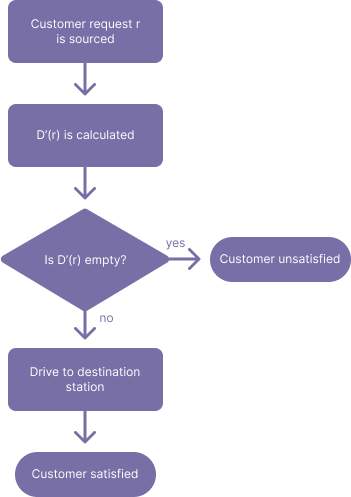
\includegraphics[width=.5\linewidth]{./Figures/event-flow.png}
  \caption{Simulation flow}
  \label{fig:Flow}
\end{figure}

A discrete-event simulation is employed, as described in Figure \ref{fig:Flow}, that aims to model a typical day of operation
for the car-sharing network. A discrete event simulation is a simulation where the flow of time is not continuous but driven
by events, such as time passed. It enables a computational efficient way to model complex systems and is a good fit for the
proposed simulation. A discrete event simulation consists of processes that can interact with other processes, access and modify
shared resources and create and listen to events.

The process that a typical customer request would flow through is given by Figure \ref{fig:Flow}. The flow is started by the
event that a customer request is sourced. This event happens periodically based on the average time period of demand $p_h$, determined
beforehand by existing demand data for each hour of the day $h \in [0,24)$. The timestamp a customer request is registered with the system
is called $t_0$ from now on.

The customer then needs to make a vehicle decision based on the request $r$ and the current Substitution Effect
 $\alpha$ resulting in $D(r, \alpha)$. The framework then calculates a more restricted set of available
possible vehicle choices $D'(\text{area}(s), \alpha) = \{c \ |\ c \in D(\text{area}(s), \alpha) \land \Delta_s(t_0, c) > -C\}$ which
includes the capacity restriction mentioned in Section \ref{sub_sec:Method/Concepts/Station}. If $D'$ is an empty set, the customer
request is labeled "unsatisfied" and $r$ is added to the set of unsatisfied requests $\mathbb{UR}$. Otherwise, a random unbiased choice between the classes in 
the set $D'$ is made resulting in the chosen class $c$ and the state of the station is updated such that 
$$
\Delta_{s_{r, 0}}(t_0 + \epsilon, c) = \Delta_{s_{r, 0}}(t_0, c) - 1
$$.
 
Following this the customer starts its rental and travels to $s_{r, 1}$. This takes him an amount of time $\delta t$ given by 
$\delta t = l_r / \text{AS}$ where $AS$ (average speed) is the average speed of urban commute. This customer then reaches
station $s_{r, 1}$ at time $t_1 = t_0 + \delta t$ and increases the delta function of the target station similarly to
$$
\Delta_{s_{r, 1}}(t_1 + \epsilon, c) = \Delta_{s_{r, 1}}(t_1, c) + 1
$$.

The rental is then counted as complete, added to the set of satisfied requests $\mathbb{SR}$ and the total profit $\pi$ is increased by $\text{cost}(c, l_r)$, completing the
customer request process. One run of the simulation framework simulates a whole day and includes the station network
as a shared resource.


\subsection{Metric \& Performance}
\label{sub_sec:Method/Metrics}

Resulting in performance metrics that can give measurable insights on the dynamics of the environment and
allows to analyze the effects of the models parameters such as the Substitution Effect $\alpha$ and the
capacity restriction $C$. The presented metrics aim to be of importance for operational decision-making
and connect the results of the simulation stage to real world performance of a car-sharing network.

\vspace*{4ex}
\renewcommand\tabularxcolumn[1]{m{#1}}
\renewcommand{\arraystretch}{1.6}
\begin{center}
\centering
\begin{tabularx}{0.9\linewidth}{@{}c|c|X@{}}
  \textbf{Metric} & \textbf{Defintion} & \textbf{Description} \\
  \hline
  URR & $\frac{|\mathbb{UR}|}{|\mathbb{UR}| + |\mathbb{SR}|}$ & The \textbf{U}nsatisfied \textbf{R}equest \textbf{R}atio, eg. the ratio of unsatisfied customers to all customers \\
  $\pi$ & {--} & The total profit of the simulation, calculated as part of the simulation stage \\
  TD & $\sum_{r \in \mathbb{SR}} l_r$ & The total distance driven during the day \\
\end{tabularx}
\end{center}

\renewcommand{\arraystretch}{1}

